\documentclass[
  11pt, % 10pt - 12pt
  %letterpaper
  %indonesian
]{assignment}

% Template-specific packages
\usepackage{mathpazo} % Use the Palatino font

\usepackage{graphicx} % Required for including images
\usepackage{booktabs} % Required for better horizontal rules in tables

\usepackage{amsmath} % Math!
\usepackage{listings} % Required for insertion of code
\usepackage{enumerate} % To modify the enumerate environment

% https://castel.dev/post/lecture-notes-2/#including-inkscape-figures-in-a-latex-document
\usepackage{import}
\usepackage{xifthen}
\usepackage{pdfpages}
\usepackage{transparent}

% Pseudocodes yay
\usepackage[english,ruled]{algorithm2e}

\usepackage[pdfusetitle]{hyperref} % Required for hyperlinks

\usepackage[]{svg}

\newcommand{\incfig}[1]{%
    \def\svgwidth{\columnwidth}
    \import{./graphics/}{#1.pdf_tex}
}


\newcommand{\ipAddress}[1]{{\fontfamily{cmtt}\selectfont #1}} % IP Address custom style!

\svgsetup{inkscape=no}

% ! CUSTOM - LST Preset
\lstset{
    language=SQL,
    frame=single, % Frames
    showstringspaces=false, % Don't put marks in string spaces
    numbers=left, % Line numbers on left
    numberstyle=\tiny, % Line numbers styling
    breaklines,
    basicstyle=\fontfamily{cmtt}\selectfont\small,
    columns=fullflexible,
}


%----------------------------------------------------------------------------------------
%	ASSIGNMENT INFORMATION
%----------------------------------------------------------------------------------------

% Student name
\author{Christopher Angelo - 2440041503}
% Institute or school name
\institute{BINUS University\\ Global Class}


% Due date
\date{July 15th, 2022}
% Assignment title
\title{Final Semester Exam Answer}

% Course details
\class{Research Methodology in Computer Science (COMP6696)}
\professor{Ms.\ Irene Anindaputri Iswanto}

\timespent{4h 03m (7:31AM)}

%----------------------------------------------------------------------------------------

\begin{document}
\maketitle

%----------------------------------------------------------------------------------------
%	ASSIGNMENT CONTENT
%----------------------------------------------------------------------------------------


\section*{Question 1}

\begin{problem}
\begin{enumerate}[a.]
  \item Explain what is called as Plagiarism! What are the factors that cause plagiarism based on your opinion?
  \item Paraphrasing is one of the methods to prevent plagiarism. Explain what is paraphrasing and how to do paraphrasing!
  \item Paraphrase the paragraph:
        \textit{Paragraph omitted for brevity, shown above the answer's paragraph.}
\end{enumerate}
\end{problem}

\subsection*{Answer 1a}

Plagiarism is the act of copying another person's work as-is and presenting those works as your own. There are a number of factors that can contribute to plagiarism, including a lack of understanding of the topic on the matters, a lack of time and / or resources, or simply accidentally not knowing how to properly cite sources.

\subsection*{Answer 1b}

Generally, paraphrasing is an act of rewriting / re-representing an idea or a sentence in a way that is different from the original. This is often done to simplify complex ideas, to make them more understandable, or, in academia, to avoid plagiarism.

When paraphrasing, it is important to keep the original meaning and context intact while giving credit to the original author. To do this, you should read through the original text once, taking notes of key points that is brought up on the text. Then, without referencing / reading the original text, write a text that covers the key points in your own. Use alternate words or phrases to make the text more unique and experiment with different ways of phrasing a sentence.

\subsection*{Answer 1c}

\begin{problem}
Theft of ideas is harder to detect, less understood, yet more relevant. It involves the use of
other's ideas, concepts, methods, and engagement with the literature without citation or
acknowledgment. Extreme cases of theft of ideas include copying the manuscript's main
contribution or conceptual model and presenting it in different words without
acknowledgment. For example, Stingl and Geraldi (2017) were plagiarized by a shorter article
that consisted of a majority of their ideas written in the author's own words and, hence, not
captured by PDS\@; the plagiarism was found by chance and the journal retracted its publication
and issued an apology. This is an extreme case. Other cases are more subtle, for example,
mentioning or explaining the concept of strategic misrepresentation and not attributing it to
Flyvbjerg et al. (2009). The concept is widely known in project studies, hence plagiarizing it
signals unethical behavior or insufficient engagement with the relevant literature. Both are
unacceptable.
\end{problem}

An unnamed author has plagiarized a manuscript by Stingl and Geraldi (2017). It slipped through the PDS as the author has paraphrased the text to an extent that it does not produce a similarity link to the original manuscript. Redacting the manuscript, the journal that the manuscript was published to had issued an apology. This is one of an example of intentional theft of ideas. While it is under-researched, idea stealing may be becoming more prominent in academia. The act of including ideas, concept and methodology from another source without any acknowledgement or citation, even minor ones, falls into the said category. Doing this is unethical as it symbolizes plagiarism.

\section*{Question 2}

\begin{problem}
\begin{enumerate}[a.]
  \item Explain what is called as peer review in a seminar or journal! Explain all steps in the peer review process as shown in the picture below!

        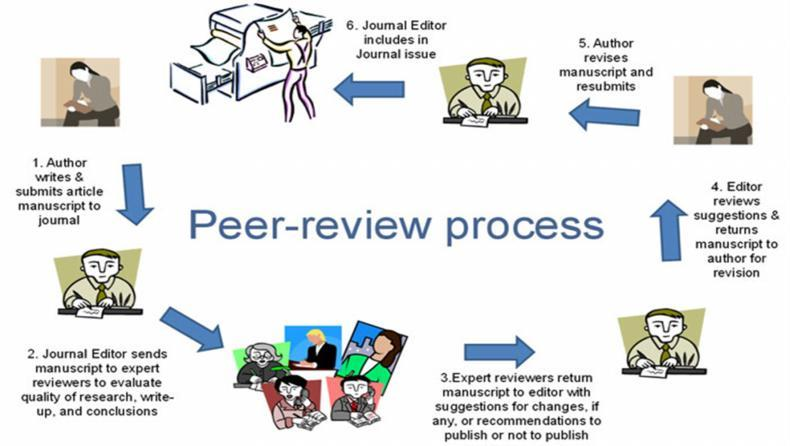
\includegraphics[width=0.9\linewidth]{graphics/20220618023028_COMP6696001_FIN_GCQuestion.jpg}

  \item One of the main aspects of reviewer's assessment is novelty. Give an example of the novelty of a reference paper used in your research (make sure the paper you use as an example is different for each group member) and explain why do you state that the paper has the novelty element. Note: Attach the paper that you used as example for this question
\end{enumerate}
\end{problem}

\subsection*{Answer 2a}

Peer review is the process of evaluating the quality of a paper submitted by a researcher. The process is divided into six steps:

\subsubsection*{Author writes \& submits article manuscript to journal}

This is essentially step 0 at the peer review process. The author would need to write the manuscript that is to be published to the journal. Usually, this would be done using a standardized paper format (i.e, IEEE) and done within a word-processing tool (i.e, \LaTeX). After this is done, the author is to submit the manuscript to a journal publication that is calling for papers.

\subsubsection*{Journal Editor sends manuscript to expert reviewers to evaluate quality of research, write-up, and conclusions}

After submiting the draft paper to the journal, the journal editor would send the paper to the expert reviewers to evaluate with an intent of writing a write-up and concluding the paper. In addition, journal editor would also check for any errors in formattings.

\subsubsection*{Expert reviewers return manuscript to editor with suggestions for changes, if any, or recommendations to publish or not to publish}

Here, the expert reviewers would check for the accuracy of the paper and the quality of the research. Optimally, the expert reviewers would not need to write a write-up and go straight to recommending on publishing. But the real world would not allow for this as mistakes happens and questions left unanswered.

\subsubsection*{Editor reviews suggestions \& returns manuscript to author for revision}

After concluding the expert's suggestions, the editor would then send the paper back to the author with the intent of revising the paper. All suggestions made by the expert reviewers and the journal editor would be incorporated in the paper which will be notified to the author.

\subsubsection*{Author revises manuscript and resubmit}

With all suggestions given back to the author, the author then would have to revise the paper and resubmit it to the journal. Every suggestion given should be acknowledged and to either revised, or left unchanged.

\subsubsection*{Journal Editor includes in Journal issue}

After the Journal Editor has done the final checking, the journal editor would then include the paper in the journal issue, thus ending the cycle of peer-review process.


\subsection*{Answer 2b}

My choice of this paper is a paper title `The Chatbot Usability Scale: the Design and Pilot of a Usability Scale for Interaction with AI-Based Conversational Agents' published by Simone Borsci et al. (2021). \href{https://link.springer.com/article/10.1007/s00779-021-01582-9}{The paper may be accessible using by clicking this sentence} (or by visiting this link: \url{https://link.springer.com/article/10.1007/s00779-021-01582-9}).

This paper is novel since it essentially creates a new measure of usability scale for conversational AI\@. It does this by combining a known usability scale that is used often to measure the user experience of a website (UMUX) and adapting an AI to them. As a result, they have created a checklist dubbed the `BOT-Check' which may be used to check the quality of a chatbot and a questionnaire dubbed `BOT Usability Scale, BUS-15' which is used to evaluate the usability of a chatbot, similar to UMUX-LITE\@.

\section*{Question 3}
\begin{problem}
\begin{enumerate}[a.]
  \item Submit the final paper of your group research work using the following IEEE template: \url{https://www.ieee.org/conferences/publishing/templates.html}
  \item Include proof of submission of your paper into an international conference / journal! Mention all the submission information detail such as:
        \begin{enumerate}[i.]
          \item The conference / journal website link
          \item Scope
          \item Organizer
          \item Date and place of event (for international conference) or Submission date (for international journal)
          \item Keynote speaker (for international conference)
        \end{enumerate}
\end{enumerate}
\end{problem}

\subsection*{Answer 3}

\begin{enumerate}
  \item \textbf{Conference} website link: \url{https://icacsis.cs.ui.ac.id}
  \item \textbf{Scope}: International
  \item \textbf{Organizer}: Universitas Indonesia
  \item \textbf{Date and place of event}:
        \begin{enumerate}[>]
          \item Submission date: July 14, 2022
          \item Event date: October 1 to 3, 2022
        \end{enumerate}
  \item \textbf{Keynote speaker}: Christopher Angelo
\end{enumerate}

\section*{Question 4}
\begin{problem}
Create a video of your paper presentation with a maximum duration of 10 minutes, then upload the video on youtube and put the url link of the youtube video in your answer. The presentation video is used to clarify the paper that has been written.
\end{problem}

\href{https://youtu.be/hwVmgV91fZg}{The following is the link to the presentation video: https://youtu.be/hwVmgV91fZg}.


\end{document}


